\section{Tractable Instances}\label{sec:tractable-queries}
CSP instances are, in general, hard to solve. To compensate for this, we may ask for characterizations of queries that are guaranteed to be efficiently solvable.

\subsection{Acyclic Queries}\label{sec:acyclic-queries}

Most work on tractable instances focuses on the concept of acyclicity. If an instance is shaped like a tree, then we may efficiently determine a solution in a single pass. Consider the three-coloring problem over this tree;

\begin{center}
\begin{tikzpicture}[level distance=1.5cm,
  level 1/.style={sibling distance=3cm},
  level 2/.style={sibling distance=1.5cm}]

% Root node
\node {A}
% First level
  child {node {B}
    % Second level
    child {node {C}}
    child {node {D}}
  }
  % First level
  child {node {E}
    % Second level
    child {node {F}}
  };

\end{tikzpicture}
\end{center}

We can start by linearly ordering the tree based on depth-first order. This specific order doesn't matter, as long as the parents come before the children.

\begin{center}
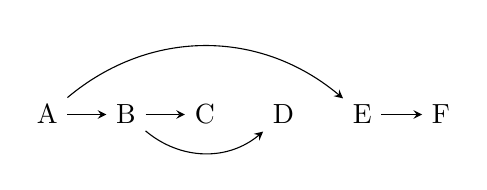
\begin{tikzpicture}[>=stealth, auto, node distance=2cm]

% Nodes
\node (A) at (0,0) {A};
\node (B) at (1,0) {B};
\node (C) at (2,0) {C};
\node (D) at (3,0) {D};
\node (E) at (4,0) {E};
\node (F) at (5,0) {F};

\draw [->] (A) -- (B);
\draw [->] (B) -- (C);
\draw [->] (E) -- (F);

\draw [->] (A) to [out=40, in=140] (E);
\draw [->] (B) to [out=320, in=220] (D);

\end{tikzpicture}
\end{center}

We can simply go in this order, making a choice of color, only needing to ensure it's consistent with the nodes that came before. Let's say we always try choosing blue, then green, then red. We assign A to blue. We move onto B, which cannot be blue, so we assign it green. We move onto C, which can be blue, so that's what we assign it. Same with D. We move onto E, which cannot be blue, so we assign it green. We may assign F to blue, so we do. We now have a complete, valid three-coloring.

\begin{center}
\begin{tikzpicture}[level distance=1.5cm,
  level 1/.style={sibling distance=3cm},
  level 2/.style={sibling distance=1.5cm}]

% Root node
\node {${\color{blue}\CIRCLE}$}
% First level
  child {node {${\color{green}\CIRCLE}$}
    % Second level
    child {node {${\color{blue}\CIRCLE}$}}
    child {node {${\color{blue}\CIRCLE}$}}
  }
  % First level
  child {node {${\color{green}\CIRCLE}$}
    % Second level
    child {node {${\color{blue}\CIRCLE}$}}
  };

\end{tikzpicture}
\end{center}

Of course, this doesn't generalize to more complex CSPs. Often, an initial choice may prevent any valid later assignments, forcing us to backtrack, which could ultimately take exponential time to find a solution. For the sake of illustration, let's assume the variable domains are restricted to the following sets.

\begin{center}
\begin{tikzpicture}[level distance=1.5cm,
  level 1/.style={sibling distance=3cm},
  level 2/.style={sibling distance=1.5cm}]

% Root node
\node {$\{{\color{blue}\CIRCLE} {\color{green}\CIRCLE} {\color{red}\CIRCLE}\}$}
% First level
  child {node {$\{{\color{green}\CIRCLE}\}$}
    % Second level
    child {node {$\{{\color{blue}\CIRCLE} {\color{red}\CIRCLE}\}$}}
    child {node {$\{{\color{blue}\CIRCLE} {\color{green}\CIRCLE} {\color{red}\CIRCLE}\}$}}
  }
  % First level
  child {node {$\{{\color{blue}\CIRCLE} {\color{green}\CIRCLE}\}$}
    % Second level
    child {node {$\{{\color{green}\CIRCLE}\}$}}
  };

\end{tikzpicture}
\end{center}

If we started by assigning A to blue, we'd eventually get a contradiction, as E would have to be assigned to green, leaving no consistent assignment for F. We modify our procedure to go in reverse first, filtering out values for the parent that are incompatible with all possibilities. This is called "arc consistency".
% ; see section \ref{sec:arc-consistency} for more details.

We start with F which must be green, so E cannot contain green. E would then be restricted to $\{{\color{blue}\CIRCLE}\}$, meaning this must be filtered from the options of A. The next is D, which implies no restrictions on B. We then go to C which also implies no restrictions on B since both options are compatible with all possibilities in B. We then move onto B, which must be green, and so that possibility is filtered from A. After this backward sweep, we have

\begin{center}
\begin{tikzpicture}[level distance=1.5cm,
  level 1/.style={sibling distance=3cm},
  level 2/.style={sibling distance=1.5cm}]

% Root node
\node {$\{{\color{red}\CIRCLE}\}$}
% First level
  child {node {$\{{\color{green}\CIRCLE}\}$}
    % Second level
    child {node {$\{{\color{blue}\CIRCLE} {\color{red}\CIRCLE}\}$}}
    child {node {$\{{\color{blue}\CIRCLE} {\color{green}\CIRCLE} {\color{red}\CIRCLE}\}$}}
  }
  % First level
  child {node {$\{{\color{blue}\CIRCLE}\}$}
    % Second level
    child {node {$\{{\color{green}\CIRCLE}\}$}}
  };

\end{tikzpicture}
\end{center}

And applying the forward sweep, we'd have the following three-coloring.

\begin{center}
\begin{tikzpicture}[level distance=1.5cm,
  level 1/.style={sibling distance=3cm},
  level 2/.style={sibling distance=1.5cm}]

% Root node
\node {${\color{red}\CIRCLE}$}
% First level
  child {node {${\color{green}\CIRCLE}$}
    % Second level
    child {node {${\color{blue}\CIRCLE}$}}
    child {node {${\color{blue}\CIRCLE}$}}
  }
  % First level
  child {node {${\color{blue}\CIRCLE}$}
    % Second level
    child {node {${\color{green}\CIRCLE}$}}
  };

\end{tikzpicture}
\end{center}

This does generalize to other CSPs; so long as our instances are tree-shaped, we can evaluate them efficiently. Cyclicity itself does not prevent us from solving a problem efficiently, though there is a sense in which the more tree-like a problem can be framed, the more efficiently it can be solved. See section \ref{sec:csp-decomposition} for details.

\subsection{CSP Decomposition}\label{sec:csp-decomposition}

Trees are not the only efficiently solvable instances. There is a large body of research focusing on characterizing efficient instances. Work on giving a full characterization will be described in section \ref{sec:complete-tractable-query-languages}. Immediately, we end up with two separate issues; identifying if a query can be cast as an efficiently solvable problem, and actually solving it. In general, it may be as hard to frame the problem properly as it would be to solve using more brute-force methods. The field of CSP decomposition is dedicated to studying efficient methods for both transforming and solving queries. Each generally defines some notion of cyclicity (the exact definition will vary based on the method), and will guarantee a solution time that is polynomial in the size of the problem while being exponential in the cyclicity measure. See \citep{gottlob2000comparison} for details and a comparison of different methods.

To demonstrate a simple method, consider this graph for the three coloring problem from section \ref{sec:three-coloring};

\begin{center}
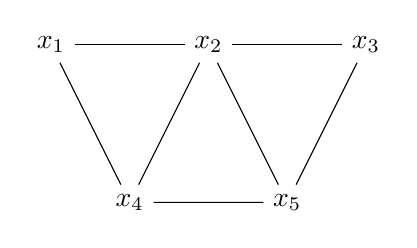
\begin{tikzpicture}
  \node (A) at (0,0) {$x_1$};
  \node (B) at (2,0) {$x_2$};
  \node (C) at (4,0) {$x_3$};
  \node (D) at (1,-2) {$x_4$};
  \node (E) at (3,-2) {$x_5$};

  \draw (A) -- (B) -- (C);
  \draw (A) -- (D) -- (E) -- (C);
  \draw (D) -- (B);
  \draw (E) -- (B);
\end{tikzpicture}
\end{center}

This is clearly not a tree. But, consider the following clusterings of variables;

\begin{center}
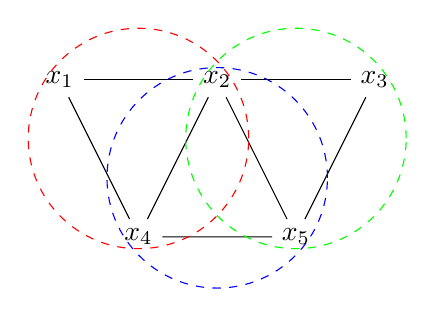
\begin{tikzpicture}
  \node (A) at (0,0) {$x_1$};
  \node (B) at (2,0) {$x_2$};
  \node (C) at (4,0) {$x_3$};
  \node (D) at (1,-2) {$x_4$};
  \node (E) at (3,-2) {$x_5$};

  \draw (A) -- (B) -- (C);
  \draw (A) -- (D) -- (E) -- (C);
  \draw (D) -- (B);
  \draw (E) -- (B);

  % Draw circles around triangles
  \draw[red, dashed] (1, -0.75) circle [radius=1.4];
  \draw[blue, dashed] (2,-1.25) circle [radius=1.4];
  \draw[green, dashed] (3, -0.75) circle [radius=1.4];

\end{tikzpicture}
\end{center}

Now, we'll use these clusters to define three new variables; $x_{124} = (x_1, x_2, x_4)$, $x_{245} = (x_2, x_4, x_5)$, and $x_{235} = (x_2, x_3, x_5)$, whose domain is the permutations of three colors,

\begin{equation}
    ColorPerms =
    \{{\color{blue}\CIRCLE} {\color{green}\CIRCLE} {\color{red}\CIRCLE}, 
    {\color{green}\CIRCLE} {\color{blue}\CIRCLE} {\color{red}\CIRCLE},
    {\color{red}\CIRCLE} {\color{green}\CIRCLE} {\color{blue}\CIRCLE},
    {\color{blue}\CIRCLE} {\color{red}\CIRCLE} {\color{green}\CIRCLE}, 
    {\color{red}\CIRCLE} {\color{blue}\CIRCLE} {\color{green}\CIRCLE},
    {\color{green}\CIRCLE} {\color{red}\CIRCLE} {\color{blue}\CIRCLE}
    \}
\end{equation}

We also have constraints relating the values of shared variables between different clusters. For our problem, the important constraints are

\begin{equation}
    E^{23}_{12} = \{((x, y, z), (y, z, w))\ |\ (x, y, z), (y, z, w) \in ColorPerms\}
\end{equation}

\begin{equation}
    E^{13}_{13} = \{((x, y, z), (x, w, z))\ |\ (x, y, z), (x, w, z) \in ColorPerms\}
\end{equation}

Using these, we can reformulate our CSP into

\begin{equation}
    E^{23}_{12}(x_{124}, x_{245}) \wedge E^{13}_{13}(x_{245}, x_{235})
\end{equation}

This is clearly tree-like. In fact, it doesn't even branch; it's a line. As such, we can now solve it efficiently. Applying the forward pass from the previous section, we can start by assigning;

\begin{equation}
    x_{124} = {\color{blue}\CIRCLE} {\color{green}\CIRCLE} {\color{red}\CIRCLE}
\end{equation}

We can then use $E^{23}_{12}$ to see that the remaining options for $x_{245}$ are

\begin{equation}
    \{{\color{green}\CIRCLE} {\color{red}\CIRCLE} {\color{blue}\CIRCLE}
    \}
\end{equation}

forcing a single option. Using this along with $E^{13}_{13}$ we can restrict $x_{235}$ to the same set. This means we have;

\begin{equation}
    x_{124} = (x_1, x_2, x_4) = {\color{blue}\CIRCLE} {\color{green}\CIRCLE} {\color{red}\CIRCLE}
\end{equation}
\begin{equation}
    x_{245} = (x_2, x_4, x_5) = {\color{green}\CIRCLE} {\color{red}\CIRCLE} {\color{blue}\CIRCLE}
\end{equation}
\begin{equation}
    x_{235} = (x_2, x_3, x_5) = {\color{green}\CIRCLE} {\color{red}\CIRCLE} {\color{blue}\CIRCLE}
\end{equation}

We can then use this solution to fill in the graph colors, obtaining;

\begin{center}
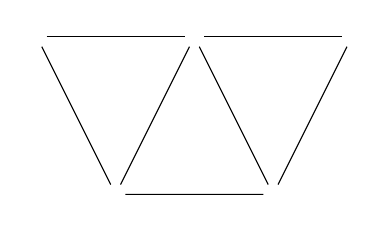
\begin{tikzpicture}
  \node (A) at (0,0) {${\color{blue}\CIRCLE}$};
  \node (B) at (2,0) {${\color{green}\CIRCLE}$};
  \node (C) at (4,0) {${\color{red}\CIRCLE}$};
  \node (D) at (1,-2) {${\color{red}\CIRCLE}$};
  \node (E) at (3,-2) {${\color{blue}\CIRCLE}$};

  \draw (A) -- (B) -- (C);
  \draw (A) -- (D) -- (E) -- (C);
  \draw (D) -- (B);
  \draw (E) -- (B);
\end{tikzpicture}
\end{center}

It's worth thinking about the complexity of this approach. Assuming we can cluster variables so that they form a tree, the time complexity will be linear with respect to the size of the clusters. However, the domains of the cluster variables will be, in general, exponentially larger than the domains we started with. This means the complexity scales exponentially with respect to cluster size. So long as the clusters can be kept manageable, the instance can be solved in a reasonable amount of time.

The most general known method for cluster creation in such a way that the resulting query is efficiently solvable is called "fractional hypertree decomposition"; see \citep{grohe2014constraint} for technical details, and see \citep{marx2013tractable} for a broader overview.

\subsection{Complete Tractable Query Languages}\label{sec:complete-tractable-query-languages}

Rather than starting with a difficult in general CSP which we then filter to tractable instances, it may be prudent to try designing a query language capable of expressing exactly and only the tractable instances for any CSP. This problem is "Gurevich’s Problem" \citep{gurevich1985logic}, and is, in its most general form, still open.

The most famous positive result is the Immerman-Vardi theorem \citep{immerman1982relational}. This states that a query language generated by relational calculus plus a least fixed point operator defines a language for queries that are exactly the queries computable in polynomial time. A variant of this stating that "the restriction of second-order logic to formulae whose first order part is a universal Horn formula” captures all P-time queries over ordered structures was proven in \citep{gradel1991expressive}.

\begin{remark}
Note that least-fixed-point logic is essentially just bare Datalog.
\end{remark}

The limitation of this is the requirement for total ordering. What this means is that some total ordering must be definable from the relations given in the CSP. An example of a poly-time query not expressible without a total ordering is the parity of an unordered set (determining if the number of elements in a set is even or odd). An unordered set corresponds to a trivial CSP where one has a domain but no actual relations. Counting the size of the domain, then the parity of that size, is clearly efficiently doable. If one had a total ordering, they could associate numbers with each element of the domain and the query would just calculate the highest element, according to this relation. Without such a relation, the query isn't expressible.

An intrinsic ordering isn't present on arbitrary graphs. If the graph is canonicalized, then this canonicalization implies an intrinsic ordering. The existence of a polynomial time graph canonization algorithm is still open; it is known to be doable in quasi-polynomial time \citep{wiebking2021decomposition}.

The goal is to create a query language whose expressive power is independent of how the model graph is laid out in memory. The only major candidates are a logic called “Choiceless Polynomial Time”, and extensions of it. Specifically, the variant with the ability to count is the minimal, still possible candidate \citep{blass1999choiceless}.

CPT with counting is essentially the weakest logic such that all queries are in PTime and there are no known PTime queries that are not expressible in it.

The basic idea of the logic is to extend the language of relations with the following abilities, intended to manipulate sets of solutions to define new relations;

\begin{itemize}
\item Take the unions of sets.
\item Take unordered pairs of sets.
\item Determine if a solution is unique (e.g. map $\{b\}$ onto $b$ and everything else onto $\{\}$).
\item Count the number of elements in a set.
\item Taking the iterated compositions of definable relations.
\end{itemize}

The semantics of the language is further mediated by providing an explicit polynomial during evaluation for the sake of limiting compute time.

% The rest of this section is dedicated to describing this logic.

% The core syntactic datastructure of the logic is a notion of a "Hereditarily Finite Set". This can mean several different things depending on the context, but for the purposes of CPT, it extends a set of (uninterpreted) relation symbols, $\tau$, using the syntax given in \ref{fig:hf_syntax}.

% \begin{figure}[!htb]
% \begin{equation*}
% \begin{array}{rclr}
%     \text{HF} &::= 
%     &| R(\text{HF}, \text{HF}, ..., \text{HF}) \text{for each} R \in \tau&\\
%     &| \emptyset&\\
%     &| &\text{Atoms}&\\
%     &| &\#(\text{HF}) &\\
%     &| &\bigcup \text{HF} &\\
%     &| &\{\text{HF},\ \text{HF}\} &\\
%     &| &\text{Unique}(\text{HF}) &\\
% \end{array}
% \end{equation*}
% \caption{Hereditarily Finite Set syntax grammar.}
% \label{fig:hf_syntax}
% \end{figure}

% Given a set of atoms, $A$, and an interpretation for $\tau$ mapping relations onto sets of tuples, HF has the interpretation stated in figure \ref{fig:hf_semantics}.

% \begin{figure}[!htb]
%     \centering
% \begin{equation*}
% \begin{array}{lclr}
%     \evalT{ \emptyset} &:\equiv &\{\} &\\
%     \evalT{ \text{Atoms}} &:\equiv &A &\\
%     \evalT{ \# a} &:\equiv &     \begin{cases}
%         0 & \text{if } \evalT{a} \in A\\
%         |\evalT{a}| \text{encoded as an ordinal} & \text{else}
%     \end{cases} &\\
%     \evalT{ \bigcup a} &:\equiv &\{b\ |\ \exists c \in \evalT{a}. b \in c\} &\\
%     \evalT{ \{a, b\}} &:\equiv &\{\evalT{a}, \evalT{b}\} &\\
%     \evalT{ \text{Unique}(a)} &:\equiv &     \begin{cases}
%         b & \text{if } \evalT{a} = \{b\}\\
%         \{\} & \text{else}
%     \end{cases} &\\
% \end{array}
% \end{equation*}
%     \caption{Hereditarily Finite Set semantics.}
%     \label{fig:hf_semantics}
% \end{figure}

There is much ongoing research trying to separate this logic from P. There are also attempts to minimally extend CPT so that its canonization invariance is more explicit. The most promising is Choiceless Polynomial Time with Witnessed Symmetric Choice \citep{lichter2022choiceless}. Also see that paper for a more detailed, streamlined presentation of regular CPT.

